\documentclass[12pt, twocolumn]{article}
\usepackage[utf8]{inputenc}
\usepackage[spanish]{babel}
\usepackage{geometry}
\geometry{a4paper,margin=0.8in}
\usepackage{amsmath}
\usepackage{listings}
\usepackage{graphicx}
\usepackage{float}
\usepackage{url}
\usepackage{booktabs}
\usepackage{amsfonts}
\usepackage{fancyhdr}
\usepackage{amssymb}
\usepackage{gensymb}
\pagestyle{fancy}
\cfoot{Página \thepage}
\lstset{basicstyle=\small\ttfamily,columns=fullflexible}

\begin{document}
	\title{TP Final: Análisis del sistema trampolín/cuerpo rígido \\ 
		   \large{\textsc{Simulación de Sistemas}} \\
		   \normalsize{\textsc{Instituto Tecnológico de Buenos Aires}}}
	\author{
		\textsc{Saqués}, M. Alejo \\
		\texttt{56047} 
		\and
		\textsc{Raies}, Tomás A. \\
		\texttt{56099}
		\and
		\textsc{Marcantonio}, Nicolás \\
		\texttt{56288}
	}
	\date{}
	\maketitle
	
	\begin{abstract}
	Se ha estudiado el sistema trampolín/cuerpo rígido mediante simulaciones implementadas en el lenguaje CUDA/C++, utilizando diversos métodos de integración y analizando la conservación de la energía de los mismos.
	
	Se ha propuesto un método de modelado de cuerpos rígidos utilizando una construcción con resortes de constante elástica acorde. Se ha estudiado la deformación del cuerpo rígido en función de dicha constante y de la cantidad de masas enlazadas.
	
	Por último, se han analizado los picos de altura alcanzados por cuerpos rígidos con diferentes orientaciones, probando que pérdidas de energía por rotaciones inducen picos de altura más bajos.
	\end{abstract}
	
	\paragraph{Palabras clave: Cuerpo rígido, \textbf{CUDA/C++} método de integración, \textit{Verlet}, \textit{RK4}, colisión.}
	
	\section{Introducción}
	
	\paragraph{} El objetivo de este trabajo fue el de estudiar algunas características relevantes del sistema trampolín/cuerpo rígido, aprovechando la eficiencia de una implementación en unidades de procesamiento gráfico (GPU).
	
	\paragraph{} Se discutirá el modelo matemático subyacente en dicha implementación, exhibiendo maquetas que permitan comprender la construcción tanto del trampolín como del cuerpo rígido. Asimismo, se detallarán las ecuaciones matemáticas que describen las fuerzas aplicadas a cada tipo de partícula, incluyendo detalles sobre cómo se realizan los cómputos en la arquitectura presentada por el lenguaje CUDA/C++.
	
	\paragraph{} En la sección de experimentación, se elaborará sobre tres temáticas: una de ellas vinculada a la conservación de la energía utilizando diferentes métodos de integración expuestos por la Cátedra, mientras que las otras dos hacen referencia a la construcción del modelo propuesto y a propiedades interesantes de los cuerpos rígidos.
	
	\section{Modelo e implementación}
	
	\paragraph{} A continuación, se describirá el modelo matemático elegido para representar el sistema estudiado en este trabajo. Adicionalmente, se explicarán los puntos centrales acerca de la implementación realizada, haciendo énfasis en las ventajas de la \textit{computación de propósito general en unidades de procesamiento gráfico} (GPGPU por sus siglas en inglés) para este tipo de problemas.
	
	\subsection{Modelo matemático}
	
	\paragraph{} Al modelo matemático se lo puede analizar en tres secciones: modelización y fuerzas aplicadas a partículas del trampolín, fuerzas entre partículas del cuerpo rígido e interacción entre partículas del trampolín y el cuerpo rígido.
	
	\subsubsection{Modelización y fuerzas entre partículas del trampolín}
	
	\paragraph{} El trampolín ha sido modelizado como una grilla bidimensional de partículas de igual radio y masa, separadas por una distancia $L$ establecida por el usuario, enlazadas a sus ocho vecinos con resortes de constante elástica $k_{grid}$. Las dimensiones de la grilla también son parametrizables.
	
    \begin{figure}[H]
		\centering
		\includegraphics[width=7cm]{schemas/grid.png}
		\caption{Esquema del modelo de la grilla}
		\label{gridschema}
	\end{figure}
	
	\paragraph{} Las fuerzas aplicadas a cada partícula de pueden subdividir en elásticas y viscosas. Las fuerzas elásticas siguen la Ley de Hooke:
	
	\begin{align}
	    F_{el(i,j)} = -k_{grid}*(d_{(i,j)}-L)*\Vec{r}_{i,j}
	\end{align}
	
	\paragraph{} Donde $k_{grid}$ es la constante elástica del resorte entre partículas vecinas de la grilla, $d_{(i,j)}$ es la distancia entre la partícula $i$ y la partícula $j$ de la grilla, $L$ es la elongación natural del resorte (i.e., la separación entre partículas de la grilla fijada por el usuario) y $\Vec{r}_{i,j}$ es el versor relativo entre $i$ y $j$. Se debe notar que esta fuerza se calcula entre cada partícula de la grilla y sus ocho vecinos, siendo los bordes del trampolín fijos. 
	
	\paragraph{} Por otro lado, las fuerzas viscosas siguen una forma proporcional a la velocidad de la partícula, según la fórmula:
	
	\begin{align}
	    F_{vi(i)} = -b_{grid}*\Vec{V}.
	\end{align}
	
	\paragraph{} Donde $b_{grid}$ es la constante viscosa de la grilla, y $\Vec{V}$ es el vector velocidad de la partícula. Nuevamente, a los bordes de la grilla no se les aplica fuerzas de ningún tipo. 
	
	\subsubsection{Modelización y fuerzas entre partículas del cuerpo rígido}
	
	\paragraph{} El cuerpo rígido se ha modelado como una serie de masas de radio $r$, unidas por resortes donde $k_{rigid} \gg k_{grid}$. Siendo $N$ es la cantidad de partículas, si $i < N-1$, la partícula $p_{i}$ está unida con $p_{i+1}$, y si $i > 0$, dicha partícula también está unida con $p_{i-1}$. Si $i = 0 \land N > 2$, $p_{0}$ está vinculada también con $p_{N-1}$. Nótese que si $L$ es la separación entre dos sucesivas masas, las partículas de los extremos están unidas por un resorte de longitud natural $L(N-1)$.
	
    \begin{figure}[H]
		\centering
		\includegraphics[width=7cm]{schemas/masses.png}
		\caption{Esquema del modelo del cuerpo rigido}
		\label{masseschema}
	\end{figure}
	
	\paragraph{} El objetivo es que el cuerpo rígido preserve su forma, es decir, que las masas no se separen del eje que las une. Debe notarse que la distancia entre partículas, el radio, la masa y dicha constante elástica son parametrizables. Por otro lado, no se ha contemplado una fuerza viscosa propia de un movimiento en medios gaseosos.
	
	\subsubsection{Colisiones entre partículas del trampolín y del cuerpo rígido}
	
	\paragraph{} Las colisiones entre partículas pueden dividirse en normales y tangenciales. Las fuerzas normales siguen la forma:
	
	\begin{align}
	   F_{N(i,j)} = -k_{n}\:\xi_{i,j}\:\Vec{n}_{i,j} \\
	   \xi_{i,j} = R_{i} + R_{j} - \left\lVert\Vec{r}_i-\Vec{r}_j  \right\rVert
	\end{align}
	
	\paragraph{} Es la fuerza normal sobre la partícula $i$ debido a una colisión con la partícula $j$, donde $k_{n}$ es una constante elástica del resorte hipotético, $R_{i}$ y $R_{j}$ son los respectivos radios, $\Vec{r}_{i}$ y $\Vec{r}_{j}$ son las respectivas posiciones, y $\Vec{n}_{i,j}$ es el versor normal.
	
	\paragraph{} Las fuerzas tangenciales se definen de la siguiente forma:
	
	
	\begin{align}
	   F_{T(i,j)} = -k_{t}\:\xi_{i,j}\:[(\Vec{v}_{i}-\Vec{v}_{j})\:\Vec{t}_{i,j}]\:\Vec{t}_{i,j}
	\end{align}
	
	\paragraph{} Es la fuerza tangencial sobre la partícula $i$ debido a una colisión con la partícula $j$, donde $k_{t}$ es una constante elástica del resorte hipotético, $\Vec{v}_{i}$ y $\Vec{v}_{j}$ son los respectivos vectores velocidad, y $\Vec{t}_{i,j}$ es el versor tangencial.
	
	\subsection{Implementación}
	
	\paragraph{} Como se ha mencionado, la implementación del algoritmo de la simulación ha sido realizada en \textbf{CUDA/C++}, utilizando el concepto GPGPU, que prevé la utilización de la arquitectura masivamente paralela de las unidades de procesamiento gráfico para aplicaciones de índole general.
	
	\paragraph{} El concepto GPGPU se basa en la implementación de funciones conocidas como \textit{kernels}, nombre que surge de las matrices de convolución habitualmente utilizadas en aplicaciones gráficas. Estos \textit{kernels} son unidades de código ejecutadas paralelamente por unidades de procesamiento de alto \textit{throughput} como son las GPUs y que, a discreción del programador, pueden ser aplicadas a unidades de datos tales como a los píxeles de una imagen, a \textit{partículas en una grilla}, etc.
	
	\paragraph{} Es preciso señalar que este tipo de implementaciones es ideal en casos en los que se debe realizar un pequeño número de cómputos en una gran cantidad de datos mutuamente independientes. Esto se debe a que las unidades de procesamiento gráficas generalmente priorizan una cantidad masiva de núcleos de procesamiento en detrimento de la velocidad de \textit{clock} de cada uno.
	
	\paragraph{} En el caso de las partículas de la grilla, por ejemplo, es posible computar para cada partícula la sumatoria de las fuerzas elásticas tomando la posición actual de la misma y de sus ocho vecinos, sabiendo que las posiciones se actualizan más tarde con algún método de integración elegido. 
	
	\subsubsection{\textbf{CUDA/C++}}
	
	\paragraph{} Siguiendo en las líneas de la temática GPGPU, se puede comenzar por introducir algunos aspectos arquitecturales básicos del lenguaje CUDA y de la declaración e invocación de \textit{kernels} en dicho lenguaje. A continuación se presenta una declaración de ejemplo (un \textit{kernel} que computa las fuerzas elásticas para cada partícula respecto de sus ocho vecinos, y aplica una fuerza viscosa):
	
    \begin{lstlisting}[linewidth=\columnwidth,breaklines=true,language=C++]
    __global__ void gridElasticForce
    (Grid<Particle> * grid, float k, float b, float natural);
    \end{lstlisting}
    
    \paragraph{} En esta función, la única palabra clave proveniente de CUDA es la palabra \verb|__global__|, que indica que la función puede únicamente ser invocada desde el \textit{host}, y que ejecutará en el \textit{device}. Es decir, la función será invocada desde el CPU (\textit{host}) para ejecutar en la GPU (\textit{device}). Debe notarse que, en la función señalada, el puntero a la grilla debe residir en la memoria global de la GPU (\textit{device}), por lo cual el programador deberá encargarse de copiar información de estructuras entre \textit{host} y \textit{device} y viceversa.
    
    \paragraph{} Ahora bien, el lector podrá preguntarse cómo se realiza esta invocación desde el CPU. Un \textit{kernel} en CUDA se ejecuta de la siguiente forma:
    
    \begin{lstlisting}[linewidth=\columnwidth,breaklines=true,language=C++]
    gridElasticForce<<<Dg,Db,Ns,S>>>(grid_device, k, b, natural);
    \end{lstlisting}
    
    \paragraph{} Donde:
    
    \begin{itemize}
        \item \verb|Dg (dim3)| especifica las dimensiones de la \textbf{grilla (grid)}
        \item \verb|Db (dim3)| especifica las dimensiones del \textbf{bloque (block)}
        \item \verb|Ns (size_t)| especifica la cantidad de \textit{bytes} a asignar dinamicamente en la memoria compartida \textit{por bloque}.
        \item \verb|S (cudaStream_t)| especifica el \textit{stream} asociado
    \end{itemize}
    
    \paragraph{} De estos conceptos, los utilizados en la implementación han sido los primeros 2. A continuación sigue una gráfica que ejemplifica dichos conceptos:
    
    \begin{figure}[H]
		\centering
		\includegraphics[width=8cm]{schemas/grid-block-exec.jpg}
		\caption{Esquema de invocación de \textit{kernels}}
		\label{gridblockexec}
	\end{figure}
	
	\paragraph{} Como se puede ver en la Figura \ref{gridblockexec}, desde el CPU se invoca un \textit{kernel}, el cual invoca de manera bloqueante en el GPU. En el GPU, dicho \textit{kernel} es ejecutado por todos los \textbf{threads} contenidos en todos los \textbf{blocks} de la \textbf{grid}, y cada \textbf{thread} tiene información distintiva que le permite ejecutar sobre una unidad de información:
	
	\begin{itemize}
	    \item \verb|blockDim (dim3)| especifica las dimensiones del \textbf{block}
	    \item \verb|blockIdx (dim3)| especifica la posición del \textbf{block} dentro de la \textbf{grid}
	    \item \verb|threadIdx (dim3)| especifica la posición del \textbf{thread} dentro del \textbf{block}
	\end{itemize}
	
    \begin{figure}[H]
		\centering
		\includegraphics[width=8cm]{schemas/dimensions.png}
		\caption{Ejemplo de dimensiones}
		\label{dimensionsexample}
	\end{figure}
	
	\paragraph{} Con esta información, es posible calcular los índices \verb|x| e \verb|y| sobre los cuales ejecutará un \textit{kernel} en un thread dado:
	
	\begin{lstlisting}[linewidth=\columnwidth,breaklines=true,language=C++]
	int x = blockIdx.x*blockDim.x + threadIdx.x;
	int y = blockIdx.y*blockDim.y + threadIdx.y;
    \end{lstlisting}
    
    \paragraph{} Luego será solo cuestión de aplicar las operaciones deseadas.
    
    \begin{figure}[H]
		\centering
		\includegraphics[width=8cm]{schemas/area.png}
		\caption{Área a tomar en cuenta para computar colisiones con el cuerpo rígido}
		\label{area}
	\end{figure}
    
    \paragraph{} Como nota adicional, este esquema ofrece versatilidad desde el punto de vista de cómo se aplica. Por ejemplo, para computar las colisiones entre el cuerpo rígido y la grilla, no es necesario considerar toda la superficie de la grilla (\ref{area}), basta con analizar únicamente la superficie de partículas por debajo del cuerpo rígido, aplicando un \textit{kernel} con los parámetros adecuados.
	
	\section{Experimentación}
	
	
	\subsection{Métodos de integración y conservación de la energía}
	\paragraph{} Para el estudio del problema, se decidió implementar distintos métodos de integración para las ecuaciones del movimiento de las partículas, en busca del integrador que se comportara de la forma más estable frente a las condiciones del sistema.
	
	\paragraph{} Se decidió ahondar en la conservación de la energía de la cama elástica bajo condiciones ideales de fricción nula, quitando las masas que reboten sobre ella. La única fuerza (aparte de los resortes) que ejerce sobre el sistema es la gravedad. Como el sistema esta ahora compuesto por múltiples oscilaciones armónicas sin disipación, es esperable que la energía total del sistema se mantenga constante a lo largo del tiempo.
	
	\paragraph{} Los integradores que se escogieron para este estudio fueron los métodos de \textit{Euler}, \textit{Velocity Verlet} y \textit{Runge-Kutta 4}. Fueron escogidos por la simplicidad de su implementación y su popularidad dentro de la literatura relacionada. 
	
	\paragraph{} Los parámetros utilizados en las simulaciones fueron los siguientes, variando únicamente la elección del método de integración:
	\begin{itemize}
        \item \textbf{tiempo simulado}=  $120\:s$
        \item \textbf{$\Delta_{t}$}= $0.001\:s$
        \item \textbf{filas}= $32$
        \item \textbf{columnas}= $32$
        \item \textbf{separación horizontal en la grilla}= $0.05\:m$
        \item \textbf{masa de partículas de la grilla}= $0.01\:kg$
        \item \textbf{radio de partículas de la grilla}= $0.02\:m$
        \item \textbf{g}= $9.81\:\frac{m}{s^2}$
        \item \textbf{k grilla}= $3000\:\frac{N}{m}$
        \item \textbf{b grilla}= $0\:\frac{kg}{s}$
	\end{itemize}
	
	\begin{figure}[H]
		\centering
		\includegraphics[width=8cm]{energy/eulerEnergy.png}
		\caption{Energía cinética más elástica: \textit{Euler}}
		\label{energy1}
	\end{figure}
	
	\begin{figure}[H]
		\includegraphics[width=8cm]{energy/verletEnergy.png}
		\caption{Energía cinética más elástica: \textit{Velocity Verlet}}
		\label{energy2}
		\centering
	\end{figure} 
	
	\begin{figure}[H]
		\centering
		\includegraphics[width=8cm]{energy/rk4Energy.png}
		\caption{Energía cinética más elástica: \textit{Runge-Kutta 4}}
		\label{energy3}
	\end{figure}
	
	\paragraph{} Como se puede ver en las figuras \ref{energy1}, \ref{energy2} y \ref{energy3}, todos los integradores experimentaron variaciones sustanciales de energía a lo largo del tiempo. \textit{Runge-Kutta 4} fue el método que perdió energía más rápidamente, mientras que \textit{Euler} y \textit{Velocity Verlet} mantuvieron un ritmo de pérdida relativamente constante luego de una pérdida inicial más pronunciada en los primeros segundos.
	
	\subsection{Análisis de la deformación del cuerpo rígido}
	
	\paragraph{} Como medida de referencia para el análisis de la deformación del cuerpo rígido, se propuso medir para cada \textit{frame} la razón entre la distancia de los extremos del cuerpo rígido en estado de reposo contra su distancia efectiva. La fórmula usada fue la siguiente:
	
	\begin{align}
	   Deform = \frac{L(N-1)}{dst(\Vec{r_{0}}, \Vec{r_{N-1})}}
	\end{align}
	
	\paragraph{} Donde $L$ es la separación natural entre dos sucesivas masas, $N$ es el número de masas enlazadas, $dst$ es la función distancia y $\Vec{r_{0}}$ y $\Vec{r_{N-1})}$ son las posiciones de los extremos del cuerpo rígido. Nótese que si el cuerpo rígido no presenta deformaciones, $Deform = 1$.
	
    \begin{figure}[H]
		\centering
		\includegraphics[width=8cm]{deformation/def.png}
		\caption{Ejemplo de longitud natural vs. longitud efectiva}
		\label{natvsefec}
	\end{figure}
	
	\paragraph{} En la Figura \ref{natvsefec} se puede observar una comparación entre las dos medidas de referencia. En amarillo se muestra la longitud natural del cuerpo rígido ($L(N-1)$), mientras que en rojo la distancia efectiva entre los extremos.
	
	\paragraph{} Para este análisis únicamente se varió la constante $k_{rigid}$ de los resortes que unen a cada partícula del cuerpo rígido y la cantidad $N$ de partículas, en cuanto al resto de los parámetros se mantuvo la configuración siguiente:
	
	\begin{itemize}
        \item \textbf{método}= verlet
        \item \textbf{tiempo simulado}=  $5\:s$
        \item \textbf{$\Delta_{t}$}= $0.0001\:s$
        \item \textbf{filas}= $60$
        \item \textbf{columnas}= $60$
        \item \textbf{separación horizontal en la grilla}= $0.05\:m$
        \item \textbf{masa de partículas de la grilla}= $0.001\:kg$
        \item \textbf{radio de partículas de la grilla}= $0.02\:m$
        \item \textbf{g}= $9.81\:\frac{m}{s^2}$
        \item \textbf{k grilla}= $3\:\frac{N}{m}$
        \item \textbf{b grilla}= $0.5\:\frac{kg}{s}$
        \item \textbf{masa por partícula del cuerpo rígido}= $0.5\:kg$
        \item \textbf{radio por partícula del cuerpo rígido}= $0.15\:m$
        \item \textbf{$k_{n}$}= $1*10^5\:\frac{N}{m}$
        \item \textbf{$k_{t}$}= $1*10^3\:\frac{N}{m}$
        \item \textbf{separación entre partículas del cuerpo rígido}= $0.15\:m$
        \item \textbf{ángulo del cuerpo rígido respecto del plano}= $0\deg$
	\end{itemize}
	
	\paragraph{} Otra decisión que se tomó fue la de estudiar, para cada combinación propuesta de $k_{rigid}$ y N, la deformación máxima alcanzada y la promedio, para poder analizar cuál de las dos variables afecta más al índice de deformación propuesto.
	
	\subsubsection{$k_{rigid}\:=\:1*10^7$, $N \in \{4,\,6,\,12\}$}
	
    \begin{figure}[H]
		\centering
		\includegraphics[width=8cm]{deformation/K10000000.png}
		\caption{Deformación promedio: $k_{rigid}\:=\:1*10^7$}
		\label{def1e7}
	\end{figure}
	
	\paragraph{} En la Figura \ref{def1e7} se puede observar que, con un $k_{rigid}$ de estas magnitudes, la deformación es insignificante, dado que para 12 partículas, la deformación promedio fue de $0.003\%$ y su máximo fue $0.016\%$. En el siguiente caso, se disminuirá considerablemente el $k_{rigid}$ a los efectos de observar las variaciones en la deformación producidas por el cambio de cantidad de partículas.
	
	\subsubsection{$k_{rigid}\:=\:1*10^3$, $N \in \{4,\,8,\,12\}$}
	
    \begin{figure}[H]
		\centering
		\includegraphics[width=8cm]{deformation/K1000.png}
		\caption{Deformación promedio: $k_{rigid}\:=\:1*10^3$}
		\label{def1e3}
	\end{figure}
	
	\paragraph{} Se puede notar que la deformación promedio subió notablemente, siendo que para 4 partículas, con $k_{rigid}\:=\:1*10^7$ había un  $0.002\%$ de deformación promedio y con $k_{rigid}\:=\:1*10^3$ hay un $0.3\%$ de deformación promedio. De todas formas como puede notarse esta deformación no se comporta de manera lineal con respecto al $k_{rigid}$ elegido.
	
	
    \begin{figure}[H]
		\centering
		\includegraphics[width=8cm]{deformation/K1000MAX.png}
		\caption{Deformación máxima: $k_{rigid}\:=\:1*10^3$}
		\label{defmax1e3}
	\end{figure}
	
	\paragraph{} En cuanto a la deformación máxima , en la Figura \ref{defmax1e3} observar una tendencia  lineal respecto al número de partículas. La fórmula de la recta interpoladora obtenida es: y = 0.002705 x + 0.0281033
	
	\subsection{Alturas alcanzadas variando la orientación del cuerpo}
	
	\paragraph{} El objetivo de este experimento es evaluar las variaciones en la altura lograda por el cuerpo rígido variando la orientación del mismo, pero manteniendo la posición del centro de masa. A tal efecto, se han realizado simulaciones de caídas a diferentes alturas, variando en cada paso únicamente la orientación del cuerpo: paralelo al plano de la cama elástica, o con una elevación de $45\deg$ respecto de la misma.
	
	\paragraph{} Asimismo, se ha evaluado también las variaciones en la altura lograda por el cuerpo debido a la disipación de energía producto de sus deformaciones. Para ello, se ha experimentado variando el $k_{rigid}$, pero mantieniendo fija la altura y la orientación del cuerpo. En el último apartado de esta sección podrán verse los resultados para este caso. 
	
	\paragraph{} Los parámetros inalterados a través de las simulaciones a continuación han sido los siguientes:
	
	\begin{itemize}
        \item \textbf{método}= verlet
        \item \textbf{tiempo simulado}=  $5\:s$
        \item \textbf{$\Delta_{t}$}= $0.0001\:s$
        \item \textbf{filas}= $64$
        \item \textbf{columnas}= $64$
        \item \textbf{separación horizontal en la grilla}= $0.05\:m$
        \item \textbf{masa de partículas de la grilla}= $0.001\:kg$
        \item \textbf{radio de partículas de la grilla}= $0.02\:m$
        \item \textbf{g}= $9.81\:\frac{m}{s^2}$
        \item \textbf{k grilla}= $2500\:\frac{N}{m}$
        \item \textbf{b grilla}= $0.5\:\frac{kg}{s}$
        \item \textbf{masa por partícula del cuerpo rígido}= $0.5\:kg$
        \item \textbf{radio por partícula del cuerpo rígido}= $0.15\:m$
        \item \textbf{$k_{n}$}= $1*10^5\:\frac{N}{m}$
        \item \textbf{$k_{t}$}= $1*10^3\:\frac{N}{m}$
        \item \textbf{separación entre partículas del cuerpo rígido}= $0.15\:m$
        \item \textbf{tamaño del cuerpo rígido}= $6$
	\end{itemize}
	
	\subsubsection{Análisis variando la orientación del cuerpo}
	
	\paragraph{} Como se ha discutido previamente, en esta sección se ha experimentado variando la orientación y la altura inicial del centro de masa del cuerpo rígido, manteniendo $k_{rigid}\:=\:1*10^7\:\frac{N}{m}$.
	
	\paragraph{} Se han ejecutado 4 simulaciones, a saber:
	
	\begin{enumerate}
	    \item $h\:=\:3\:m$ y $\Theta\:=\:0\deg$
	    \item $h\:=\:3\:m$ y $\Theta\:=\:45\deg$
	    \item $h\:=\:6\:m$ y $\Theta\:=\:0\deg$
	    \item $h\:=\:6\:m$ y $\Theta\:=\:45\deg$
	\end{enumerate}
	
	\paragraph{} El siguiente gráfico muestra las evoluciones en la altura del cuerpo rígido para las simulaciones 1 y 2.
	
    \begin{figure}[H]
		\centering
		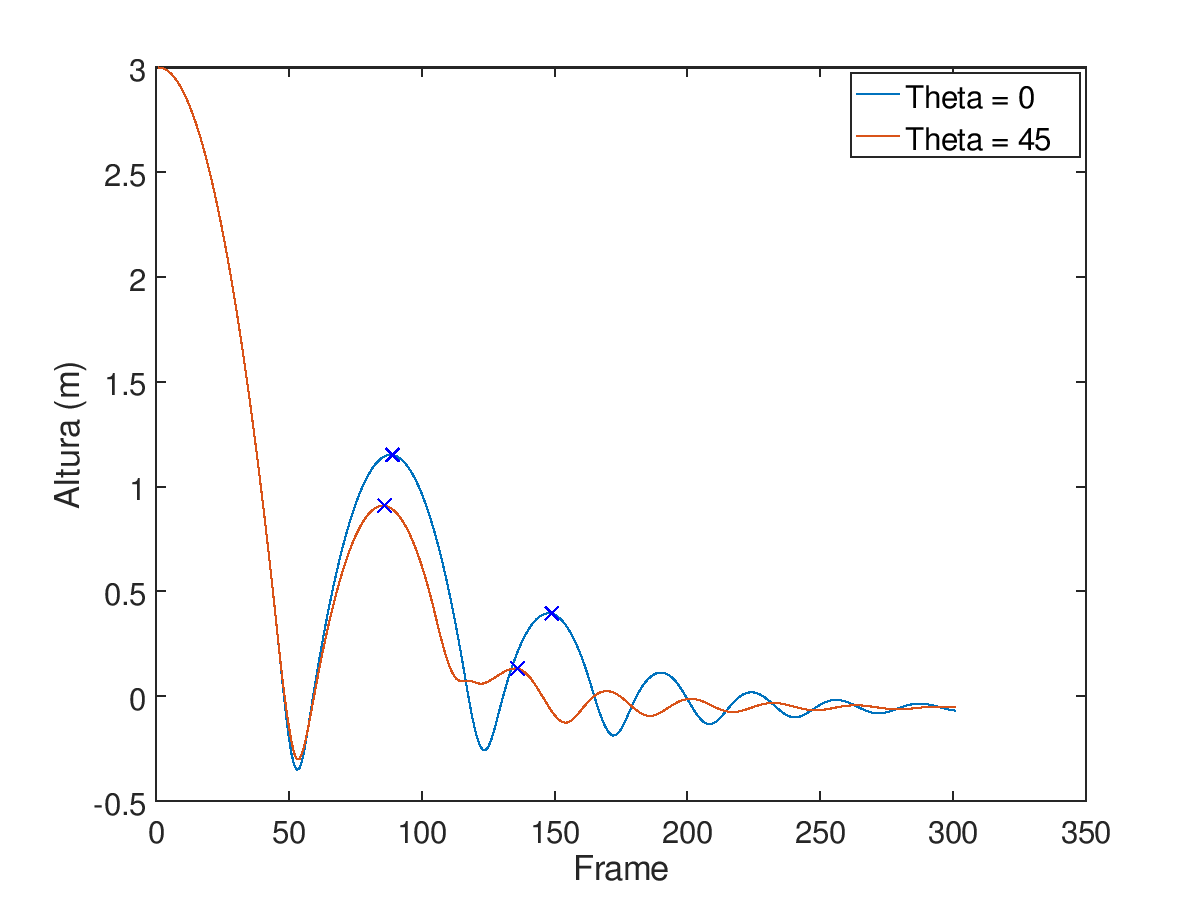
\includegraphics[width=9cm]{height/h-3-heights.png}
		\caption{Alturas logradas: simulaciones 1 y 2}
		\label{h3}
	\end{figure}
	
	\paragraph{} Como se puede observar en la Figura \ref{h3}, resulta evidente que el cuerpo colocado inicialmente paralelo al plano de la cama elástica logra picos de altura mayores al del otro caso. Para los primeros dos pares correspondientes de picos se obtuvieron las siguientes métricas:
	
    \begin{table}[H]
    \begin{tabular}{@{}lllll@{}}
    \toprule
    $max(\Theta = 0)$ & Idx & $max(\Theta = 45)$ & Idx & Rel    \\ \midrule
    1.152 m           & 89  & 0.909 m            & 86  & 1.267 \\
    0.396 m           & 149 & 0.133 m            & 136 & 2.986 \\ \bottomrule
    \end{tabular}
    \end{table}
	
	\paragraph{} Nótese que el cuerpo colocado a $45\deg$ respecto de la grilla colisiona unos instantes antes que su homólogo paralelo a la misma. Puede notarse también que este desfasaje se incrementa en el tiempo. 
	
    \begin{figure}[H]
		\centering
		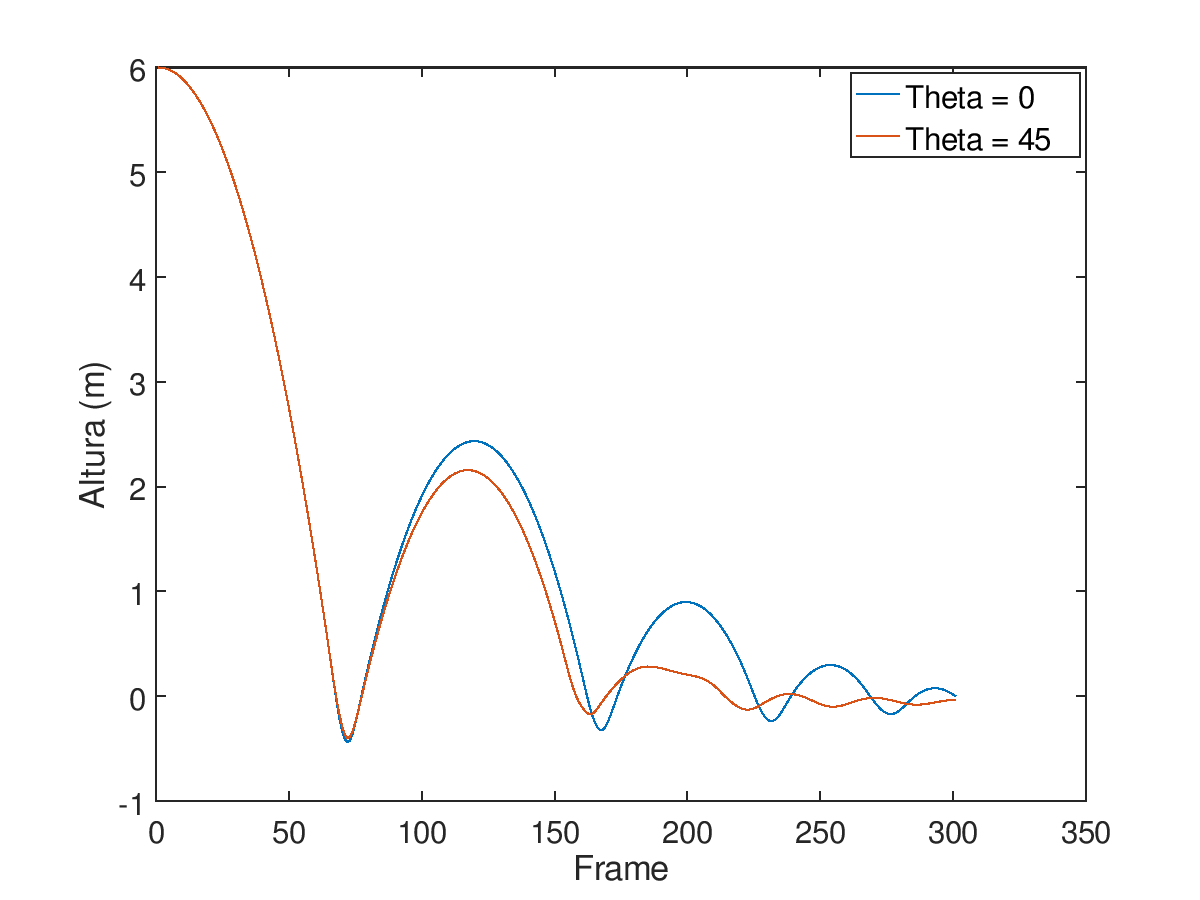
\includegraphics[width=9cm]{height/h-6-heights.png}
		\caption{Alturas logradas: simulaciones 3 y 4}
		\label{h6}
	\end{figure}
	
	\paragraph{} Este comportamiento se repite para los casos en los que $h\:=\:6\:m$ (Figura \ref{h6}). De manera similar al caso anterior, se obtuvieron las siguientes métricas para los dos primeros pares de picos de altura:
	
	\begin{table}[H]
    \begin{tabular}{@{}lllll@{}}
    \toprule
    $max(\Theta = 0)$ & Idx & $max(\Theta = 45)$ & Idx & Rel    \\ \midrule
    2.434 m           & 121 & 2.157 m             & 118 & 1.128 \\
    0.899 m           & 200 & 0.283 m            & 186 & 3.172 \\ \bottomrule
    \end{tabular}
    \end{table}
	
	\paragraph{} Como podrá notarse, las relaciones entre los máximos conservan un orden similar entre los dos pares de simulaciones. Para el primer pico, la altura del primer pico difiere en un orden del $20\%$, mientras que para el segundo, dicha diferencia se sitúa alrededor del $300\%$.
	
    \begin{figure}[H]
		\centering
		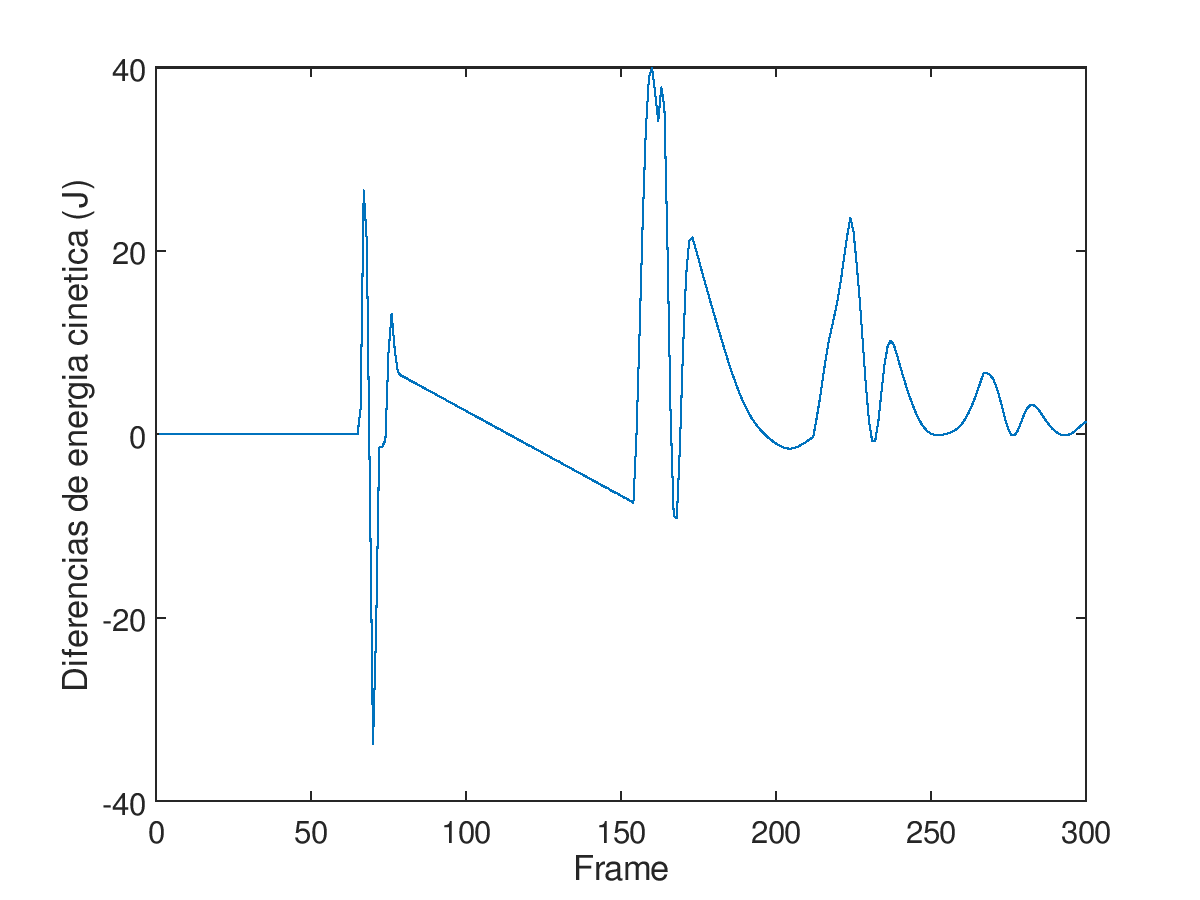
\includegraphics[width=9cm]{height/h-6-kineticDiff.png}
		\caption{Diferencia en la energía cinética entre el cuerpo no inclinado y el inclinado}
		\label{h6kineticdiff}
	\end{figure}
	
	\paragraph{} En la Figura \ref{h6kineticdiff} se observa una gráfica de la diferencia de energía cinética entre el cuerpo no inclinado y el inclinado. Es decir, cuando la gráfica es negativa, el cuerpo inicialmente inclinado tiene una sumatoria de energías cinéticas mayor a la del cuerpo inicialmente paralelo al plano del trampolín.
	
	\paragraph{} Como se podrá notar, el punto de mayor interés ocurre en el entorno de la primera colisión con el trampolín. Antes de ello, al estar imperturbados ambos cuerpos rígidos, no hay diferencias en la energía cinética de los mismos. Al colisionar, sin embargo, se puede notar que hay un transitorio de \textit{frames} en el que el cuerpo con $\Theta = 45$ adquiere una energía cinética muy superior, lo que es atribuible a la rotación del cuerpo producto de la colisión. Esto puede justificar las menores alturas alcanzadas por dicho cuerpo rígido en instantes posteriores. 
	
	\subsubsection{Análisis variando la constante elástica del cuerpo rígido}
	
	\paragraph{} Considerando que si cuerpo rígido sufre deformaciones se pierde energía en el proceso, se puede suponer que, a alturas y orientaciones iguales, pero variando ($k_{rigid}$), los picos de altura logrados varíen.
	
	\paragraph{} Para analizar esta suposición, se comparará la simulación $3$ del apartado anterior con una nueva simulación de idénticos parámetros de altura e inclinación, pero estableciendo $k_{rigid}\:=\:1*10^3\:\frac{N}{m}$. El objetivo es que, en esta nueva simulación, el cuerpo rígido sea sumamente flexible, causando así deformaciones al momento del primer impacto. Se buscará analizar si producto de estas deformaciones hay variabilidad en los máximos logrados. 
	
    \begin{figure}[H]
		\centering
		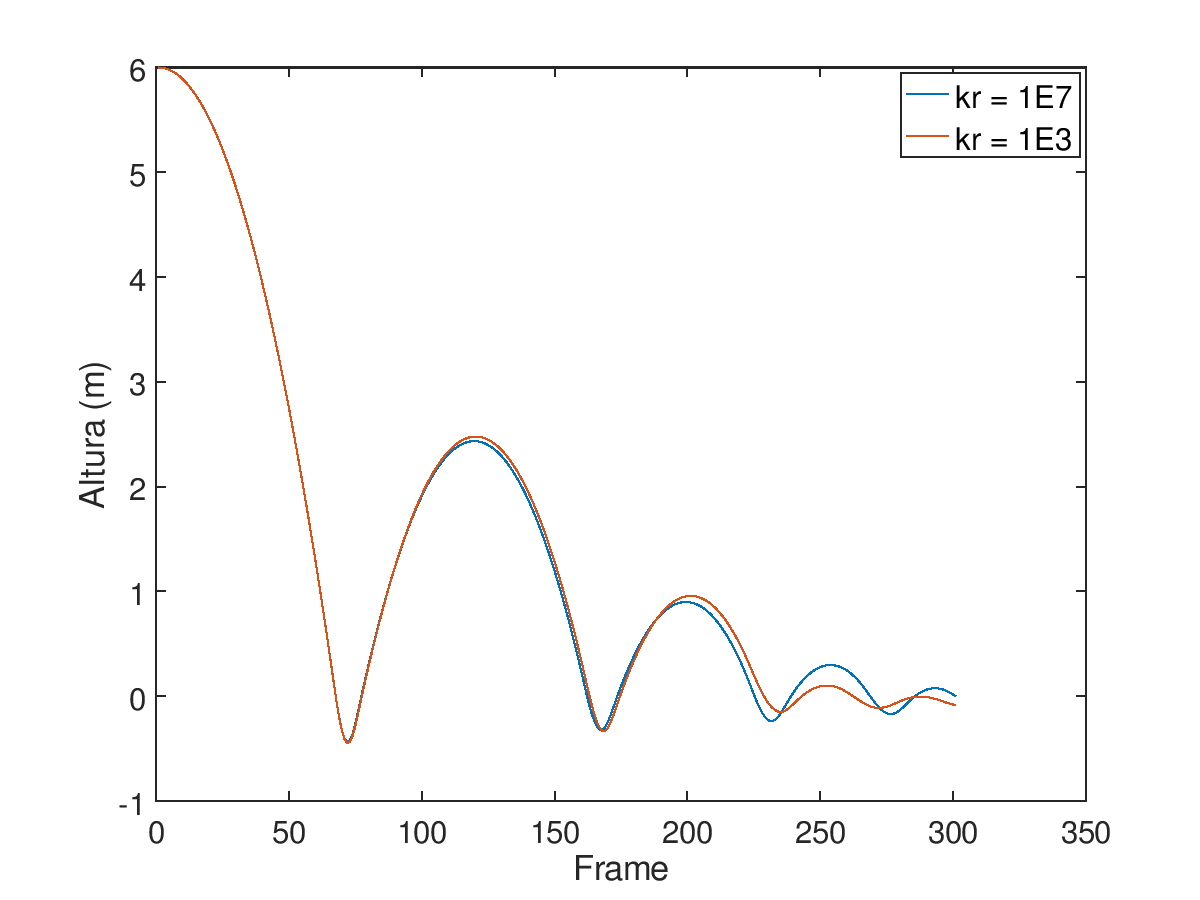
\includegraphics[width=9cm]{height/h-6-heights-E7vsE3.png}
		\caption{Alturas logradas: variación en el $k_{rigid}$}
		\label{e7ve3}
	\end{figure}
	
	
    \begin{table}[H]
    \begin{tabular}{@{}lllll@{}}
    \toprule
    $max(k_{1E7})$ & Idx & $max(k_{1E3})$ & Idx & Rel   \\ \midrule
    2.434 m         & 121 & 2.478 m          & 121 & 0.982 \\
    0.899 m         & 200 & 0.958 m          & 202 & 0.939 \\
    0.297 m         & 255 & 0.101 m          & 254 & 2.943 \\ \bottomrule
    \end{tabular}
    \end{table}
	
	\paragraph{} A diferencia de lo que pudo esperarse, se puede observar que en los dos primeros pares de casos el cuerpo con más tendencia a la deformación alcanzó alturas ligeramente por encima al de su contraparte más rígido. No obstante, en el tercer par de máximos esta tendencia se revierte abruptamente. A continuación sigue un análisis de la energía del par de cuerpos rígidos.
	
    \begin{figure}[H]
		\centering
		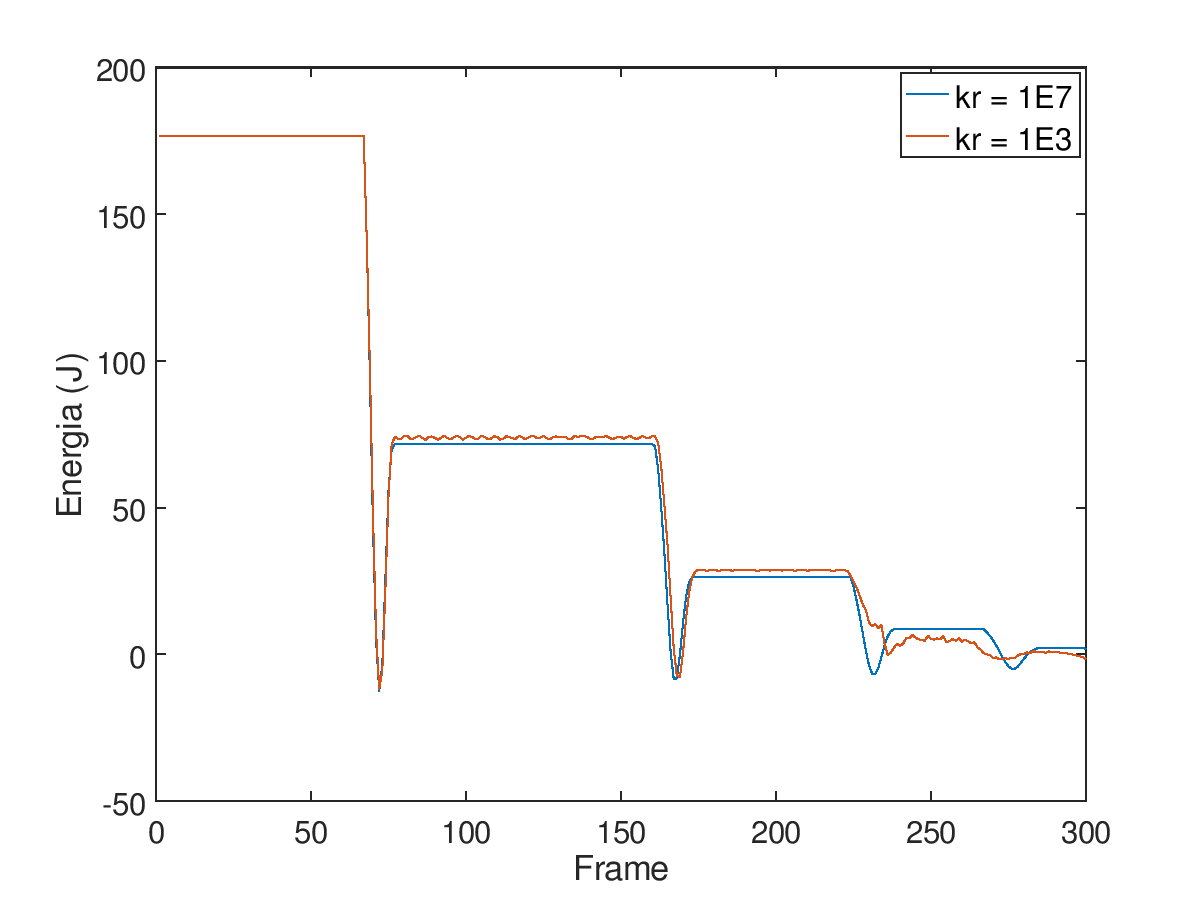
\includegraphics[width=9cm]{height/energy-1e7-1e3.png}
		\caption{Comparación de la energía total}
		\label{e7ve3en}
	\end{figure}
	
	\paragraph{} Como se podrá observar en la Figura \ref{e7ve3en}, las gráficas de la energía total (cinética y gravitatoria) de ambos casos son aproximadamente similares, siendo la del cuerpo con $k_{rigid}\:=\:1*10^3\:\frac{N}{m}$ ligeramente mayor en algunos tramos, en correspondencia con lo observado más arriba (debido a la mayor energía potencial gravitatoria en dichos tramos).
	
    \begin{figure}[H]
		\centering
		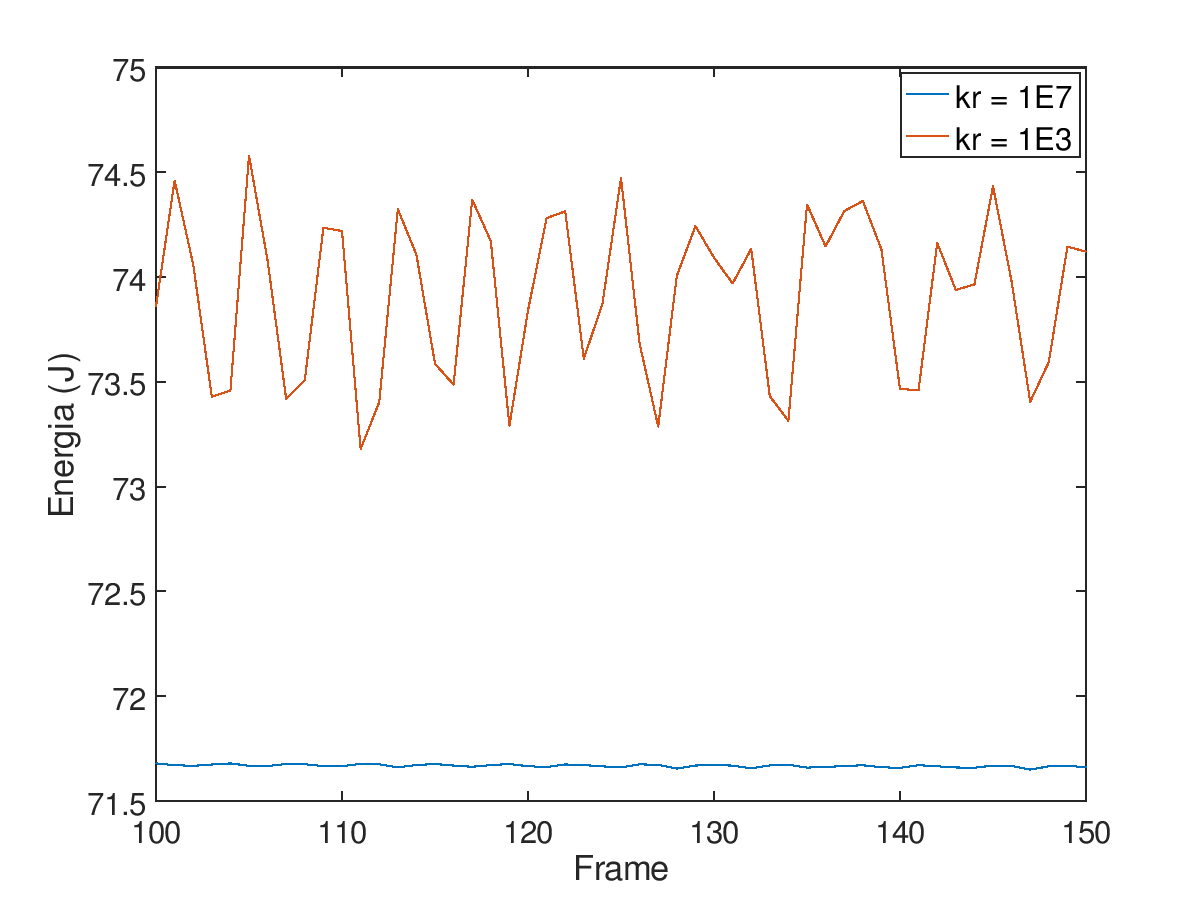
\includegraphics[width=9cm]{height/energy-detail-1e7-1e3.png}
		\caption{Detalle de la gráfica anterior}
		\label{e7ve3detail}
	\end{figure}
	
	\paragraph{} En la Figura \ref{e7ve3detail} se puede observar un detalle de la Figura \ref{e7ve3en} en el tramo entre los \textit{frames} 100 a 150. Aquí se puede ver las oscilaciones en la energía producto de las deformaciones que sufre el cuerpo rígido. 
	
	\section{Conclusiones}
	
	\paragraph{} En primer lugar, a partir de los resultados obtenidos se encontró que el método de \textit{Runge-Kutta 4} tiene mayor perdida de energía que tanto \textit{Velocity Verlet} como \textit{Euler}. Esto se deja en evidencia más fácilmente si se trabaja con sistemas sin fuerzas disipativas como el estudiado.
	
	\paragraph{} En cuanto a la deformación del cuerpo rígido, de la forma que se planteó en este trabajo, se ve más afectada por variaciones de la constante $k_{rigid}$, si bien no se ha observado una relación de tipo lineal entre esta deformación y dicha constante. Sin embargo, se notó que la deformación máxima se ve afectada por la cantidad de partículas de forma directa.
	
	\paragraph{} Por último, se ha comprobado que a iguales alturas iniciales pero diferentes orientaciones, los cuerpos rígidos alcanzan picos de altura diferentes. Se ha observado que las relaciones entre los correspondientes máximos locales de altura son similares para dos pares de cuerpos a diferentes alturas iniciales, manteniendo sus orientaciones. 

    \begin{thebibliography}{9}
        \bibitem{CUDAdesc} 
        Procesamiento paralelo CUDA
        \url{https://www.nvidia.es/object/cuda-parallel-computing-es.html}.
        
	\end{thebibliography}
	
\end{document}
